\chapter{धारा--विभव वक्र}\label{ch:b2:current-potential-curves}

इस्पात पर ज़िंक अम्लीय कुंडों से विद्युत-लेपित किया जाता है। फिर भी प्रथम वर्ष के खंड का
विभव--pH आरेख कहता है कि ज़िंक, हाइड्रोजन रेखा से बहुत नीचे होने के कारण, अम्ल का
अपचयन करके उतनी ही तेज़ी से घुल जाना चाहिए जितनी तेज़ी से वह जमता है। ऐसा नहीं होता, क्योंकि
आरेख बताता है कि क्या हो सकता है, यह नहीं कि कितनी तेज़ी से। इलेक्ट्रोड अभिक्रिया की दर
एक धारा है, और उस धारा को इलेक्ट्रोड विभव के सापेक्ष आलेखित करना
तुरंत दिखा देता है कि कौन-सी अभिक्रियाएँ तीव्र हैं, कौन-सी मंद, और कौन-सी अभिकारक की
आपूर्ति से रुकी हुई हैं। ये \omterm{def:b2:current-potential-curves:ie-curve}{धारा--विभव वक्र} हर उस विद्युत-रसायनज्ञ के साधन हैं
जो कोई धातु लेपित करता है, बैटरी आवेशित करता है या नदी में ऑक्सीजन मापता है।

\begin{recall}
प्रथम वर्ष का खंड: इलेक्ट्रोड विभव, संदर्भ इलेक्ट्रोड, नेर्न्स्ट
समीकरण, विभव--pH आरेख और उनकी सीमा (वे बताते हैं कि क्या संभव है, यह नहीं कि कितनी
तेज़ी से)। \Cref{ch:b2:cell-thermodynamics}: $\Delta_r G = -nFE$, व्युत्पन्न नेर्न्स्ट
समीकरण। भौतिकी से: विसरण और फ़िक का नियम, $j = -D\,dc/dx$।
\end{recall}

\begin{omfigure}
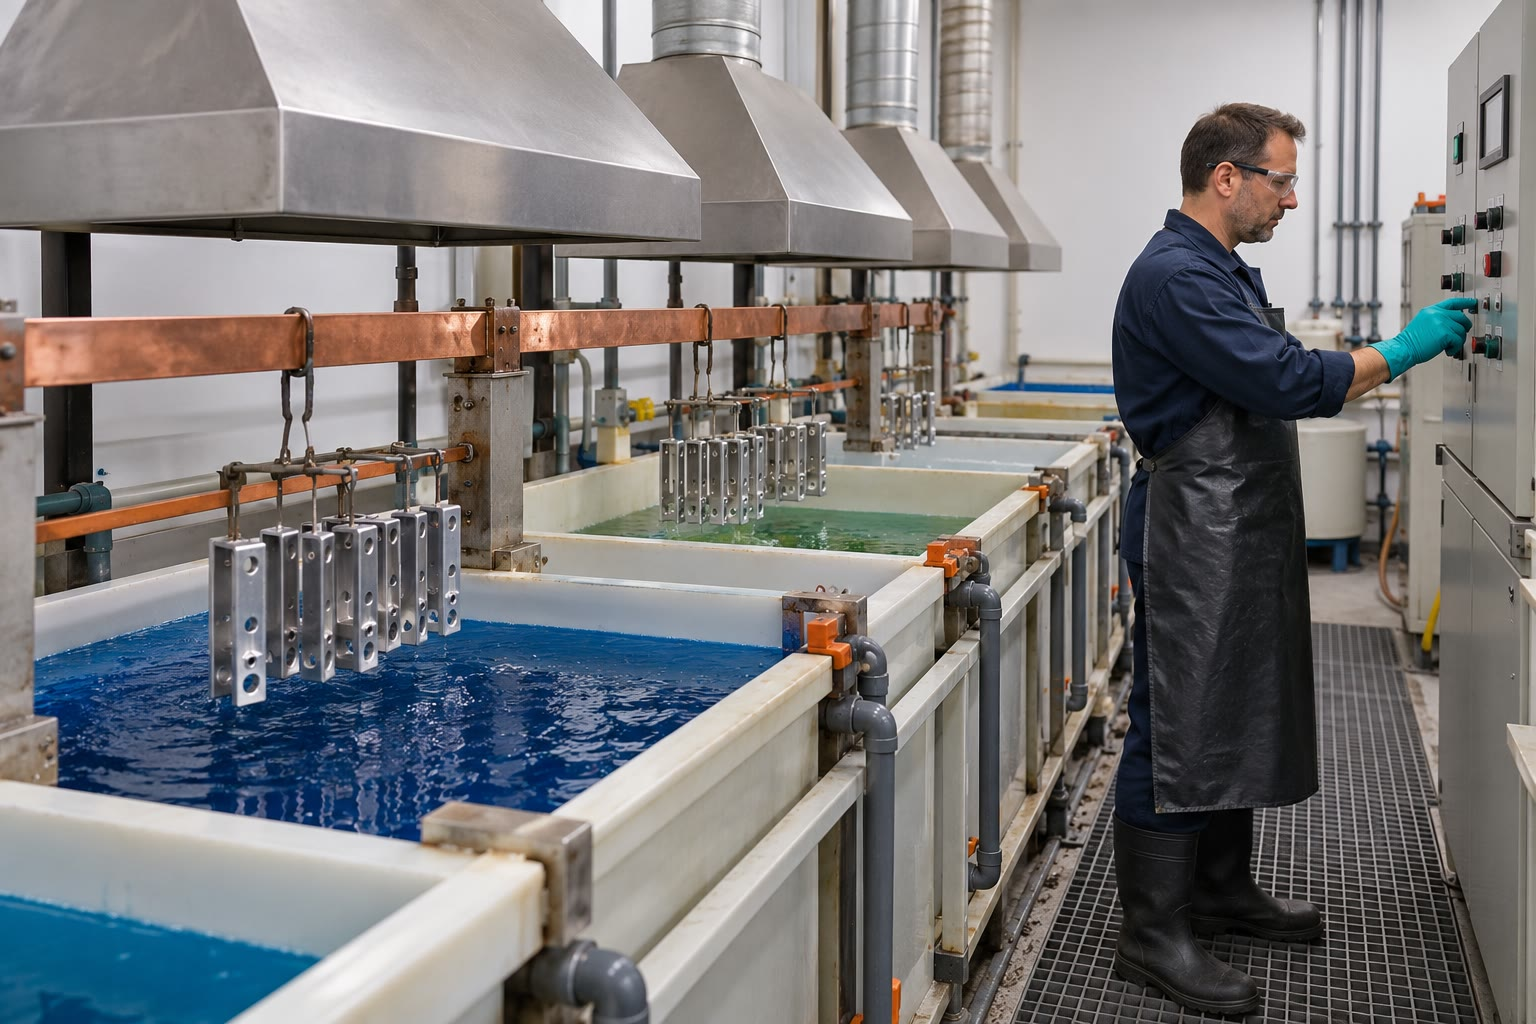
\includegraphics[width=0.62\linewidth]{images/book3/ai/b2-10-electroplating.jpg}

{\small एक विद्युत-लेपन पंक्ति: लेपित किए जाने वाले भाग ताँबे की बस-छड़ों से
कुंडों में लटकते हैं और कैथोड बनाए जाते हैं; संचालक दिष्टकारी पर धारा
तय करता है। धारा तय करती है कि धातु कितनी तेज़ी से जमती है; भागों का विभव
तय करता है कि कौन-सी धातु, या कितनी हाइड्रोजन, उसके साथ बनती है।}
\end{omfigure}

\section{साम्य से बाहर एक इलेक्ट्रोड}

\begin{definition}[धारा--विभव वक्र]\label{def:b2:current-potential-curves:ie-curve}
किसी विलयन में इलेक्ट्रोड का \emph{धारा--विभव वक्र}\index{धारा--विभव वक्र}
इलेक्ट्रोड से होकर धारा $i$ का उसके विभव $E$ के सापेक्ष आलेख है।
\emph{ऐनोडी धारा}\index{ऐनोडी धारा},
जो धनात्मक गिनी जाती है, इलेक्ट्रोड पर ऑक्सीकरण के संगत है;
\emph{कैथोडी धारा}\index{कैथोडी धारा}, जो ऋणात्मक गिनी जाती है, अपचयन के संगत।
\end{definition}

\begin{definition}[विद्युत-सक्रिय स्पीशीज़]\label{def:b2:current-potential-curves:electroactive}
\emph{विद्युत-सक्रिय स्पीशीज़}\index{विद्युत-सक्रिय स्पीशीज़} वह स्पीशीज़ है
जो विचाराधीन विभवों के परिसर में इलेक्ट्रोड पर ऑक्सीकृत या अपचित
हो सकती है।
\end{definition}

\begin{proposition}[धारा और दर]\label{prop:b2:current-potential-curves:current-rate}
यदि किसी इलेक्ट्रोड पर $n$ इलेक्ट्रॉनों वाली एक ही अर्ध-अभिक्रिया होती है, तो
धारा उसकी दर मापती है: $i = nF\,d\xi/dt$, जहाँ $\xi$ ऑक्सीकरण की प्रगति है
(जिससे ऑक्सीकरण के लिए $i > 0$, अपचयन के लिए $i < 0$)।
\end{proposition}

\begin{proof}
\cref{prop:b2:cell-thermodynamics:charge} से प्रगति $d\xi$ आवेश $nF\,d\xi$ को
इलेक्ट्रोड से होकर समय $dt$ में ले जाती है।
\end{proof}

ऐसा वक्र दर्ज करने के लिए किसी एक इलेक्ट्रोड का विभव, जब उससे धारा बह रही हो,
आरोपित और मापा जाना चाहिए --- जो दो-इलेक्ट्रोड सेल नहीं कर सकता,
क्योंकि धारा दूसरे इलेक्ट्रोड का विभव भी बदल देती है।

\begin{definition}[तीन-इलेक्ट्रोड व्यवस्था]\label{def:b2:current-potential-curves:set-up}
तीन-इलेक्ट्रोड व्यवस्था में धारा \emph{कार्यकारी
इलेक्ट्रोड}\index{कार्यकारी इलेक्ट्रोड}, जिसका अध्ययन किया जाता है, और \emph{प्रति-इलेक्ट्रोड}\index{प्रति-इलेक्ट्रोड}
के बीच बहती है, जो परिपथ पूरा करता है; कार्यकारी इलेक्ट्रोड का विभव एक संदर्भ इलेक्ट्रोड
के विरुद्ध मापा जाता है जिससे होकर कोई धारा नहीं बहती।
इलेक्ट्रॉनिक विभवस्थापी धारा को इस प्रकार समायोजित करता है कि
यह विभव आरोपित मान पर बना रहे।
\end{definition}

\begin{omfigure}
\begin{tikzpicture}[font=\small, >={Stealth}]
  \pic[transform shape] at (0,0) {beaker={0.7}{omDef!14}};
  \pic at (-0.55,0.25) {electrode={black!35}};
  \pic at (0.55,0.25) {electrode={black!15}};
  \pic (r) at (0.0,0.15) {probe};
  \draw[thick, rounded corners] (-2.2,4.3) rectangle (2.2,5.5);
  \node at (0,4.9) {विभवस्थापी};
  \draw[thick, omThm] (-0.40,2.65) -- (-0.40,3.5) -- (-1.6,3.5) -- (-1.6,4.3);
  \draw[thick, omDef] (0.70,2.65) -- (0.70,3.5) -- (1.6,3.5) -- (1.6,4.3);
  \draw[thick] (r-top) -- (0,4.3);
  \node[anchor=east, font=\scriptsize, omThm] at (-1.65,3.85) {WE};
  \node[anchor=west, font=\scriptsize, omDef] at (1.65,3.85) {CE};
  \node[anchor=west, font=\scriptsize] at (0.05,3.95) {RE};
  \draw[<-, omProp, thick] (-0.75,1.2) -- (-2.0,1.4) node[left, text=black, align=right] {कार्यकारी\\ इलेक्ट्रोड};
  \draw[<-, omProp, thick] (0.85,1.2) -- (2.1,1.4) node[right, text=black, align=left] {प्रति-\\ इलेक्ट्रोड};
  \draw[<-, omProp, thick] (0.05,0.5) -- (1.4,-0.4) node[right, text=black] {संदर्भ इलेक्ट्रोड};
  \node[font=\scriptsize, align=center] at (0,6.0) {$E_{\text{WE}} - E_{\text{RE}}$ आरोपित करता है, $i$ मापता है};
\end{tikzpicture}

{\small तीन-इलेक्ट्रोड व्यवस्था। विभवस्थापी \omterm{def:b2:current-potential-curves:set-up}{कार्यकारी इलेक्ट्रोड} (WE) और
\omterm{def:b2:current-potential-curves:set-up}{प्रति-इलेक्ट्रोड} (CE) के बीच धारा इस प्रकार चलाता है कि
संदर्भ इलेक्ट्रोड (RE) के विरुद्ध मापा गया \omterm{def:b2:current-potential-curves:set-up}{कार्यकारी इलेक्ट्रोड} का विभव
आरोपित मान पर बना रहे; संदर्भ इलेक्ट्रोड से कोई धारा नहीं
बहती।}
\end{omfigure}

जब कोई धारा नहीं बहती और किसी युग्म के दोनों रूप उपस्थित होते हैं, तो इलेक्ट्रोड
युग्म का नेर्न्स्ट विभव ले लेता है --- यदि इलेक्ट्रॉन विनिमय उसे स्थापित करने के लिए
पर्याप्त तीव्र हो। विभव को उससे हटाने पर धारा
बहने लगती है।

\section{तीव्र और मंद निकाय}

\begin{definition}[अधिविभव]\label{def:b2:current-potential-curves:overpotential}
जिस इलेक्ट्रोड से धारा $i$ बहती है, उसका \emph{अधिविभव}\index{अधिविभव}
$\eta = E(i) - E_{\text{साम्य}}$ है, अर्थात् उसके विभव और युग्म के साम्य (नेर्न्स्ट) विभव
का अंतर। किसी अर्ध-अभिक्रिया का
\emph{देहली विभव}\index{देहली विभव} वह विभव है
जिसके आगे उसकी धारा उल्लेखनीय हो जाती है।
\end{definition}

\begin{definition}[तीव्र और मंद निकाय]\label{def:b2:current-potential-curves:fast-slow}
कोई युग्म किसी दिए गए इलेक्ट्रोड पर \emph{तीव्र निकाय}\index{तीव्र निकाय} है यदि
विभव के उसके नेर्न्स्ट विभव से हटते ही उल्लेखनीय धारा बहने लगे;
वह \emph{मंद निकाय}\index{मंद निकाय} है यदि धारा के उल्लेखनीय होने से पहले, किसी भी
दिशा में, वोल्ट के कुछ दसवें भाग का \omterm{def:b2:current-potential-curves:overpotential}{अधिविभव} आवश्यक हो।
\end{definition}

कोई निकाय तीव्र है या मंद, यह युग्म और इलेक्ट्रोड के पदार्थ
पर निर्भर करता है। \ce{Fe^3+}/\ce{Fe^2+} और \ce{Ag+}/\ce{Ag} युग्म प्लैटिनम पर
तीव्र हैं; \ce{H+} का अपचयन प्लैटिनम पर तीव्र है परंतु पारे,
सीसे या ज़िंक पर मंद; जल का डाइऑक्सीजन में ऑक्सीकरण हर इलेक्ट्रोड पर मंद है।
आबंध तोड़ने या बनाने वाले इलेक्ट्रॉन स्थानांतरण, जैसे \ce{O2} या \ce{H2} वाले,
प्रायः मंद होते हैं; लगभग एक ही आकृति के दो आयनों के बीच इलेक्ट्रॉन का
स्थानांतरण तीव्र होता है। मंद वक्र के उठते भाग की आकृति इलेक्ट्रॉन स्थानांतरण की
गतिकी से आती है, जो तृतीय वर्ष के खंड में व्युत्पन्न की गई है।

\begin{omfigure}
\begin{tikzpicture}
\begin{axis}[omie, width=0.47\linewidth, height=5.4cm, xmin=0.25, xmax=1.3,
  ymin=-1.3, ymax=1.3, xlabel={$E$}, ylabel={$i$}, title={\small तीव्र निकाय}]
\addplot[omanodic] table[x=E, y=i, restrict expr to domain={\thisrow{i}}{0:2}] {figdata/out/bachelor-2-ie-curves-a.dat};
\addplot[omcathodic] table[x=E, y=i, restrict expr to domain={\thisrow{i}}{-2:0}] {figdata/out/bachelor-2-ie-curves-a.dat};
\draw[densely dotted] (axis cs:0.77,-1.2) -- (axis cs:0.77,1.2);
\node[font=\scriptsize, anchor=north west] at (axis cs:0.78,-0.05) {$E_{\text{साम्य}}$};
\node[font=\scriptsize, anchor=south] at (axis cs:1.1,1.0) {\ce{Fe^2+} $\to$ \ce{Fe^3+}};
\node[font=\scriptsize, anchor=north] at (axis cs:0.45,-1.0) {\ce{Fe^3+} $\to$ \ce{Fe^2+}};
\end{axis}
\end{tikzpicture}\hfill
\begin{tikzpicture}
\begin{axis}[omie, width=0.47\linewidth, height=5.4cm, xmin=-0.25, xmax=1.8,
  ymin=-1.3, ymax=1.3, xlabel={$E$}, ylabel={$i$}, title={\small मंद निकाय}]
\addplot[omanodic] table[x=E, y=i, restrict expr to domain={\thisrow{i}}{0:2}] {figdata/out/bachelor-2-ie-curves-c.dat};
\addplot[omcathodic] table[x=E, y=i, restrict expr to domain={\thisrow{i}}{-2:0}] {figdata/out/bachelor-2-ie-curves-c.dat};
\draw[densely dotted] (axis cs:0.77,-1.2) -- (axis cs:0.77,1.2);
\draw[<->, omProp] (axis cs:0.77,0.5) -- (axis cs:1.12,0.5) node[midway, above, font=\scriptsize] {$\eta_a$};
\draw[<->, omProp] (axis cs:0.42,-0.5) -- (axis cs:0.77,-0.5) node[midway, below, font=\scriptsize] {$\eta_c$};
\node[font=\scriptsize, anchor=north west] at (axis cs:0.78,-0.05) {$E_{\text{साम्य}}$};
\end{axis}
\end{tikzpicture}

{\small ऐसे युग्म के मॉडल \omterm{def:b2:current-potential-curves:ie-curve}{धारा--विभव वक्र} जिसके दोनों रूप समान सांद्रताओं में
उपस्थित हैं (ऐनोडी शाखा लाल, कैथोडी नीली)। बाएँ, एक \omterm{def:b2:current-potential-curves:fast-slow}{तीव्र
निकाय}: साम्य विभव पर धारा तीव्रता से चिह्न बदलती है। दाएँ,
एक \omterm{def:b2:current-potential-curves:fast-slow}{मंद निकाय}: उसके आसपास विभवों के एक परिसर में कोई धारा नहीं बहती; हर
शाखा को \omterm{def:b2:current-potential-curves:overpotential}{अधिविभव} चाहिए। दोनों समान सीमांत पठारों तक पहुँचते हैं, जो
विसरण से तय होते हैं। (निदर्शी मान।)}
\end{omfigure}

\section{द्रव्य परिवहन और सीमांत धाराएँ}

जब इलेक्ट्रॉन स्थानांतरण तीव्र हो, तो धारा इलेक्ट्रोड पर अभिकारक के पहुँचने से
सीमित होती है। विलोडित विलयन में इलेक्ट्रोड से सटी द्रव की एक पतली परत
लगभग स्थिर रहती है, और अभिकारक उसे विसरण द्वारा
पार करता है।

\begin{definition}[विसरण परत और सीमांत धारा]\label{def:b2:current-potential-curves:limiting-current}
\emph{विसरण परत}\index{विसरण परत} इलेक्ट्रोड से सटी विलयन की वह परत है,
मोटाई $\delta$ वाली (विलोडित विलयन में कुछ से लेकर कुछ दसियों माइक्रोमीटर),
जिसके आर-पार स्पीशीज़ केवल विसरण द्वारा
चलती हैं। \emph{सीमांत धारा}\index{सीमांत धारा} वह धारा है
जो तब प्राप्त होती है जब \omterm{def:b2:current-potential-curves:electroactive}{विद्युत-सक्रिय स्पीशीज़} उतनी ही तेज़ी से उपभुक्त होती है जितनी तेज़ी से वह पहुँचती है, और
सतह पर उसकी सांद्रता शून्य होती है।
\end{definition}

\begin{omfigure}
\begin{tikzpicture}[font=\small, >={Stealth}, x=1.2cm, y=1.2cm]
  \fill[black!25] (-0.4,0) rectangle (0,3);
  \node[rotate=90, font=\scriptsize] at (-0.2,1.5) {इलेक्ट्रोड};
  \draw[->] (0,0) -- (4.6,0) node[right] {$x$};
  \draw[->] (0,0) -- (0,3.2) node[above] {$c$};
  \draw[densely dashed] (1.6,0) -- (1.6,3);
  \node[below, font=\scriptsize] at (1.6,0) {$\delta$};
  \draw[omDef, thick] (0,1.2) -- (1.6,2.4) -- (4.4,2.4);
  \draw[omThm, thick] (0,0.02) -- (1.6,2.4);
  \node[font=\scriptsize, anchor=west] at (2.6,2.6) {स्थूल, $c^b$ (विलोडित)};
  \node[font=\scriptsize, omDef, anchor=east] at (-0.45,1.2) {$c^s$};
  \node[font=\scriptsize, omThm, anchor=west] at (1.7,0.5) {$c^s = 0$: सीमांत धारा};
  \node[font=\scriptsize, align=center] at (0.8,3.0) {विसरण\\ परत};
\end{tikzpicture}

{\small विलोडित विलयन में इलेक्ट्रोड के निकट अभिकारक की सांद्रता।
\omterm{def:b2:current-potential-curves:limiting-current}{विसरण परत} के आर-पार प्रोफ़ाइल रैखिक है; अभिवाह, और इसलिए
धारा, $c^b - c^s$ के समानुपाती है। यह तब अधिकतम होती है जब अभिकारक
पहुँचते ही उपभुक्त हो जाता है ($c^s = 0$, लाल)।}
\end{omfigure}

\begin{theorem}[सीमांत धारा]\label{thm:b2:current-potential-curves:limiting}
स्थूल सांद्रता $c$ और विसरण गुणांक $D$ वाली किसी स्पीशीज़ के लिए,
जो मोटाई $\delta$ की \omterm{def:b2:current-potential-curves:limiting-current}{विसरण परत} को पार करके क्षेत्रफल $A$ के इलेक्ट्रोड तक पहुँचती है,
\omterm{def:b2:current-potential-curves:limiting-current}{सीमांत धारा}, निरपेक्ष मान में, यह है:
\[
  |i_{\lim}| = \frac{nFADc}{\delta} .
\]
\end{theorem}

\begin{proof}
स्थायी अवस्था में परत में सांद्रता प्रोफ़ाइल रैखिक है (फ़िक का
द्वितीय नियम $\partial c/\partial t = 0$ के साथ $d^2c/dx^2 = 0$ देता है), अतः इलेक्ट्रोड
की ओर अभिवाह $j = D(c - c^s)/\delta$ है, मोल प्रति इकाई क्षेत्रफल और
समय में। पहुँचने वाला हर अणु $n$ इलेक्ट्रॉनों के साथ अभिक्रिया करता है: $|i| = nFAj =
nFAD(c - c^s)/\delta$, जो $c^s = 0$ के लिए अधिकतम है।
\end{proof}

\begin{example}[सीमांत धारा का परिमाण]\label{ex:b2:current-potential-curves:ilim}
\qty{10}{mmol/L} (\qty{10}{mol/m^3}) वाली किसी स्पीशीज़ के लिए, $D =
\qty{7e-10}{m^2/s}$, $\delta = \qty{20}{\micro m}$, $n = 1$ के साथ,
\qty{1.0}{cm^2} पर: $|i_{\lim}| = 96\,485 \times 10^{-4} \times 7 \times 10^{-10}
\times 10/(2 \times 10^{-5}) = \qty{3.4}{mA}$।
\end{example}

\begin{theorem}[तीव्र निकाय की तरंग]\label{thm:b2:current-potential-curves:wave}
किसी तीव्र युग्म $\mathrm{Ox} + n\,\mathrm e^- \rightleftharpoons \mathrm{Red}$ के लिए,
ऐनोडी \omterm{def:b2:current-potential-curves:limiting-current}{सीमांत धारा} $i_{\lim,a} > 0$ (Red द्वारा तय) और कैथोडी
\omterm{def:b2:current-potential-curves:limiting-current}{सीमांत धारा} $i_{\lim,c} < 0$ (Ox द्वारा तय) के साथ, स्थायी अवस्था का वक्र यह है:
\[
  E = E_{1/2} + \frac{RT}{nF}\ln\frac{i - i_{\lim,c}}{i_{\lim,a} - i},
  \qquad E_{1/2} = E^\circ + \frac{RT}{nF}\ln\frac{D_{\text{Red}}}{D_{\text{Ox}}} ,
\]
जहाँ परत की मोटाई दोनों रूपों के लिए समान है।
\end{theorem}

\begin{proof}\emergencystretch=3em
\omterm{def:b2:current-potential-curves:fast-slow}{तीव्र निकाय}: सतह पर नेर्न्स्ट समीकरण लागू होता है, $E = E^\circ + (RT/nF)
\ln(c^s_{\text{Ox}}/c^s_{\text{Red}})$। रैखिक प्रोफ़ाइल: \omterm{def:b2:current-potential-curves:ie-curve}{ऐनोडी धारा} $i$
सतह पर Red का उपभोग करती है और Ox बनाती है, $i = nFAD_{\text{Red}}(c^b_{\text{Red}}
- c^s_{\text{Red}})/\delta = -nFAD_{\text{Ox}}(c^b_{\text{Ox}} - c^s_{\text{Ox}})/\delta$।
$i_{\lim,a} = nFAD_{\text{Red}}c^b_{\text{Red}}/\delta$ और $i_{\lim,c} =
-nFAD_{\text{Ox}}c^b_{\text{Ox}}/\delta$ के साथ इनसे $c^s_{\text{Red}} = (i_{\lim,a} -
i)\delta/(nFAD_{\text{Red}})$ और $c^s_{\text{Ox}} = (i - i_{\lim,c})\delta/(nFAD_{\text{Ox}})$ मिलते हैं।
नेर्न्स्ट समीकरण में रखिए।
\end{proof}

\begin{corollary}[अर्ध-तरंग विभव]\label{cor:b2:current-potential-curves:half-wave}
जब दोनों रूपों के विसरण गुणांक बराबर हों, तो $E_{1/2} = E^\circ$: जब
केवल एक रूप उपस्थित हो, तो युग्म के मानक विभव पर धारा अपने सीमांत मान की
आधी होती है।
\end{corollary}

\begin{proof}
केवल Red उपस्थित होने पर $i_{\lim,c} = 0$, और $i = i_{\lim,a}/2$ के लिए लघुगणक
शून्य हो जाता है: $E = E_{1/2} = E^\circ$ जब $D_{\text{Red}} = D_{\text{Ox}}$।
\end{proof}

\begin{proposition}[पठार सांद्रताएँ मापते हैं]\label{prop:b2:current-potential-curves:plateau}
नियत विलोडन और इलेक्ट्रोड पर, किसी पठार की ऊँचाई उस स्पीशीज़ की
सांद्रता के समानुपाती होती है जिसका वह उपभोग करता है: पठार पर किसी विभव पर
रखा गया इलेक्ट्रोड एक ऐम्पियरमितीय संवेदक है।
\end{proposition}

\begin{proof}
$|i_{\lim}| = (nFAD/\delta)\,c$, और कोष्ठक का गुणक नियत
विलोडन और ताप पर स्थिर है।
\end{proof}

\begin{omfigure}
\begin{tikzpicture}
\begin{axis}[omie, width=0.47\linewidth, height=5.0cm, xmin=0.25, xmax=1.3,
  ymin=-0.3, ymax=1.3, xlabel={$E$}, ylabel={$i$}, title={\small केवल \ce{Fe^2+} उपस्थित}]
\addplot[omanodic] table[x=E, y=i] {figdata/out/bachelor-2-ie-curves-b.dat};
\draw[densely dotted] (axis cs:0.77,0) -- (axis cs:0.77,0.5) -- (axis cs:0.25,0.5);
\node[font=\scriptsize, anchor=north] at (axis cs:0.77,-0.02) {$E_{1/2}$};
\node[font=\scriptsize, anchor=south west] at (axis cs:0.27,0.5) {$i_{\lim}/2$};
\node[font=\scriptsize, anchor=south] at (axis cs:1.12,1.0) {पठार};
\end{axis}
\end{tikzpicture}\hfill
\begin{tikzpicture}
\begin{axis}[width=0.42\linewidth, height=5.0cm, xmin=0, xmax=1.05, ymin=0, ymax=1.1,
  axis x line=bottom, axis y line=left, xtick=\empty, ytick=\empty,
  xlabel={$c$}, ylabel={$i_{\lim}$}, label style={font=\small},
  title={\small ऐम्पियरमिति}]
\addplot[omanodic, mark=*, mark size=1.2pt] table[x=c, y=i] {figdata/out/bachelor-2-ie-curves-e.dat};
\end{axis}
\end{tikzpicture}

{\small बाएँ: तीव्र युग्म की तरंग जब केवल अपचित रूप उपस्थित हो
(मॉडल); उसकी आधी ऊँचाई अर्ध-तरंग विभव पर है। दाएँ: पठार की
ऊँचाई सांद्रता के अनुपात में बढ़ती है।}
\end{omfigure}

\section{विलायक और इलेक्ट्रोड}

जल स्वयं विद्युत-सक्रिय है: यह डाइऑक्सीजन में ऑक्सीकृत होता है
(\ce{2H2O -> O2 + 4H+ + 4e-}) और डाइहाइड्रोजन में अपचित (\ce{2H+ + 2e- -> H2}, या
\ce{2H2O + 2e- -> H2 + 2OH-})। चूँकि विलायक कभी समाप्त नहीं होता, उसके वक्रों का
कोई पठार नहीं होता: वे तीव्रता से उठते हैं और हर अन्य वक्र को सीमित करते हैं।

\begin{definition}[विद्युत-सक्रियता खिड़की]\label{def:b2:current-potential-curves:window}
\emph{विलायक भित्तियाँ}\index{विलायक भित्ति} विलायक के ऑक्सीकरण और अपचयन
की खड़ी शाखाएँ हैं। \emph{विद्युत-सक्रियता
खिड़की}\index{विद्युत-सक्रियता खिड़की} उनके बीच विभवों का वह परिसर है
जिसमें घुली हुई स्पीशीज़ के वक्र देखे जा सकते हैं।
\end{definition}

\begin{proposition}[जल की खिड़की]\label{prop:b2:current-potential-curves:window}
दिए गए pH पर जल में खिड़की जल के दो युग्मों के ऊष्मागतिक परिसर,
$\qty{0}{V} - 0.059\,\mathrm{pH}$ और $\qty{1.23}{V} -
0.059\,\mathrm{pH}$, के आसपास होती है, जो हर ओर प्रयुक्त इलेक्ट्रोड पर संगत
अभिक्रिया के \omterm{def:b2:current-potential-curves:overpotential}{अधिविभव} से चौड़ी हो जाती है।
\end{proposition}

\begin{proof}[तर्क]
हर भित्ति अपने युग्म के नेर्न्स्ट विभव के निकट, देहली \omterm{def:b2:current-potential-curves:overpotential}{अधिविभव} से खिसककर,
आरंभ होती है: जल का ऑक्सीकरण सभी इलेक्ट्रोडों पर मंद है, इसलिए
ऐनोडी भित्ति \qty{1.23}{V} (pH 0 पर) से वोल्ट के कुछ दसवें भाग ऊपर है;
\ce{H+} का अपचयन प्लैटिनम पर तीव्र है, जिसकी कैथोडी भित्ति
\qty{0}{V} के निकट रहती है, परंतु ज़िंक, सीसे या पारे पर मंद, जिनकी भित्ति वोल्ट के
कई दसवें भाग नीचे है।
\end{proof}

\begin{omfigure}
\begin{tikzpicture}
\begin{axis}[omie, width=0.82\linewidth, height=5.4cm, xmin=-1.2, xmax=2.0,
  ymin=-3, ymax=3, xlabel={$E$ (V)}, ylabel={$i$}, clip=true, clip mode=individual]
\addplot[omwall] table[x=E, y=i] {figdata/out/bachelor-2-ie-curves-d-high.dat};
\addplot[omcathodic] table[x=E, y=i, restrict expr to domain={\thisrow{E}}{-1.2:0.6}] {figdata/out/bachelor-2-ie-curves-d-Pt.dat};
\addplot[omanodic] table[x=E, y=i, restrict expr to domain={\thisrow{E}}{0.6:2.0}] {figdata/out/bachelor-2-ie-curves-d-Pt.dat};
\draw[densely dotted] (axis cs:0,-2.8) -- (axis cs:0,2.8);
\draw[densely dotted] (axis cs:1.23,-2.8) -- (axis cs:1.23,2.8);
\node[font=\scriptsize, anchor=north west] at (axis cs:0.02,-0.1) {0};
\node[font=\scriptsize, anchor=north west] at (axis cs:1.24,-0.1) {1.23};
\node[font=\scriptsize, omDef, anchor=west] at (axis cs:0.05,-2.2) {Pt पर \ce{H+} $\to$ \ce{H2}};
\node[font=\scriptsize, gray, anchor=east] at (axis cs:-0.85,-1.0) {Zn, Pb पर};
\node[font=\scriptsize, omThm, anchor=east] at (axis cs:1.18,2.2) {\ce{H2O} $\to$ \ce{O2}};
\end{axis}
\end{tikzpicture}

{\small pH 0 पर जल की भित्तियाँ (मॉडल)। \ce{H+} का अपचयन प्लैटिनम पर
\qty{0}{V} के निकट आरंभ होता है (नीला), परंतु ज़िंक या सीसे जैसी धातुओं पर
वोल्ट के कई दसवें भाग नीचे (खंडित); जल के ऑक्सीकरण को किसी भी
इलेक्ट्रोड पर \omterm{def:b2:current-potential-curves:overpotential}{अधिविभव} चाहिए। खिड़की भित्तियों के बीच का परिसर है।}
\end{omfigure}

\section{वक्रों को पढ़ना}

\begin{method}[किसी विलयन के वक्रों का रेखाचित्र]\label{met:b2:current-potential-curves:sketch-ie}
\begin{enumerate}
  \item pH और इलेक्ट्रोड के पदार्थ के लिए विलायक की दोनों भित्तियाँ
        खींचिए।
  \item उपस्थित हर युग्म के लिए उसका नेर्न्स्ट विभव (दोनों रूप
        उपस्थित) या $E^\circ$ (एक रूप) रखिए: \omterm{def:b2:current-potential-curves:fast-slow}{तीव्र निकाय} वहाँ अक्ष को
        तीव्रता से काटता है; \omterm{def:b2:current-potential-curves:fast-slow}{मंद निकाय} अपने \omterm{def:b2:current-potential-curves:overpotential}{अधिविभवों} से खिसका होता है।
  \item हर तरंग को उस स्पीशीज़ की सांद्रता के समानुपाती पठार दीजिए
        जिसका वह उपभोग करती है; स्वयं को ऑक्सीकृत करने वाले धातु इलेक्ट्रोड का कोई
        पठार नहीं होता (धातु समाप्त नहीं होती)।
  \item हर विभव पर संभव अभिक्रियाओं की धाराएँ जोड़िए।
\end{enumerate}
\end{method}

\begin{method}[वक्रों को पढ़ना]\label{met:b2:current-potential-curves:read-ie}
\begin{enumerate}
  \item आरोपित विभव पर हर वक्र पर हर अभिक्रिया की धारा
        पढ़िए: वे साथ-साथ चलती हैं, अपनी धाराओं के अनुपात में।
  \item आरोपित धारा (विद्युत-अपघटन) पर वह विभव खोजिए जिस पर
        ऐनोडी या कैथोडी वक्र जुड़कर उस धारा के बराबर होते हैं; सम्मिलित अभिक्रियाएँ
        वे हैं जिनके वक्र वहाँ योगदान करते हैं।
  \item किसी सेल, या संक्षारित होती धातु, के लिए एक अभिक्रिया की \omterm{def:b2:current-potential-curves:ie-curve}{ऐनोडी धारा}
        दूसरी की \omterm{def:b2:current-potential-curves:ie-curve}{कैथोडी धारा} के बराबर होती है: बिंदुओं का वह युग्म
        खोजिए।
\end{enumerate}
\end{method}

\begin{example}[अम्लीय कुंड से ज़िंक लेपन]\label{ex:b2:current-potential-curves:zinc}
अम्लीय ज़िंक कुंड में कैथोड पर दो संभव अपचयन होते हैं: \ce{Zn^2+
+ 2e- -> Zn} ($E^\circ = \qty{-0.76}{V}$, तीव्र) और \ce{2H+ + 2e- -> H2}
($E^\circ = \qty{0}{V}$)। ऊष्मागतिक रूप से हाइड्रोजन पहले आनी चाहिए और ज़िंक
कभी नहीं। परंतु ज़िंक पर \ce{H+} का अपचयन मंद है: उसकी भित्ति
\qty{-0.76}{V} से नीचे है, और जिस विभव पर ज़िंक उपयोगी दर से जमता है,
वहाँ थोड़ी ही हाइड्रोजन बनती है। आरेख नहीं, वक्र
लेपन की व्याख्या करता है।
\end{example}

\begin{history}[ध्रुवणलेखन]
\begin{minipage}[t]{0.25\linewidth}
\vspace{0pt}
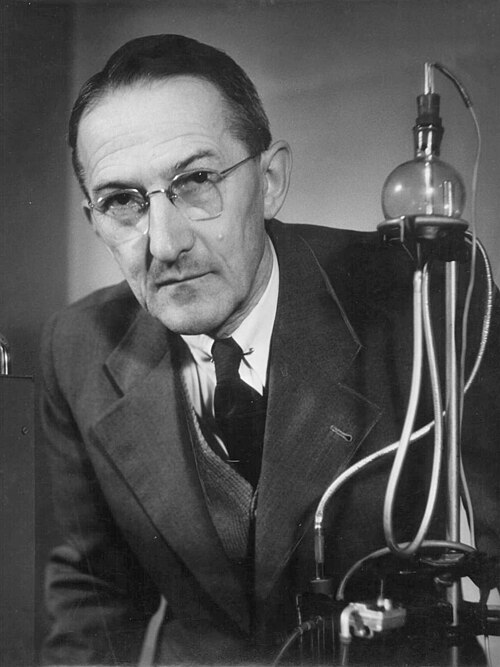
\includegraphics[width=\linewidth]{images/book3/heyrovsky.jpg}
\end{minipage}\hfill
\begin{minipage}[t]{0.71\linewidth}
\vspace{0pt}
1922 में यारोस्लाव हेयरोव्स्की ने एक पारा इलेक्ट्रोड से होकर धारा दर्ज की
जो केशिका की नोक पर बूँद-दर-बूँद बनता था, जबकि विभव को
क्रमवीक्षित किया जा रहा था: हर अपचेय स्पीशीज़ ने एक सीढ़ी दी, जिसकी स्थिति उसे पहचानती थी और
जिसकी ऊँचाई उसकी सांद्रता मापती थी। नवीकृत बूँद सतह को
ताज़ा रखती थी, और पारे पर हाइड्रोजन के ऊँचे \omterm{def:b2:current-potential-curves:overpotential}{अधिविभव} ने एक चौड़ी
कैथोडी खिड़की खोल दी। ध्रुवणलेखन के लिए उन्हें 1959 में रसायन का नोबेल पुरस्कार मिला,
और इसने विद्युत-विश्लेषी रसायन की नींव रखी; छायाचित्र में वे
टपकते-पारे इलेक्ट्रोड के साथ हैं। (छायाचित्र: जे॰~हेयरोव्स्की भौतिक रसायन
संस्थान का अभिलेखागार, CC BY-SA 3.0, विकिमीडिया कॉमन्स।)
\end{minipage}
\end{history}

\section{अभ्यास}

\begin{exercise}[$\star$]\label{exo:b2:current-potential-curves:1}
धारा देते हुए डेनियल सेल में, इस अध्याय की परिपाटियों के साथ,
ज़िंक इलेक्ट्रोड और ताँबे के इलेक्ट्रोड पर धारा का चिह्न
बताइए।
\end{exercise}

\begin{exercise}[$\star$]\label{exo:b2:current-potential-curves:2}
\ce{Ag+} (\qty{2.0}{mmol/L}, $D =
\qty{1.6e-9}{m^2/s}$) के अपचयन की \omterm{def:b2:current-potential-curves:limiting-current}{सीमांत धारा} \qty{0.50}{cm^2} पर $\delta = \qty{25}{\micro m}$ के साथ परिकलित कीजिए
(मॉडल मान)।
\end{exercise}

\begin{exercise}[$\star$]\label{exo:b2:current-potential-curves:3}
अध्याय के मॉडल वक्रों पर आप तीव्र और \omterm{def:b2:current-potential-curves:fast-slow}{मंद निकाय} को कैसे पहचानते हैं?
प्लैटिनम पर हर एक का एक उदाहरण दीजिए।
\end{exercise}

\begin{exercise}[$\star$]\label{exo:b2:current-potential-curves:4}
किसी विलयन में केवल \ce{Fe^2+} है। यदि दोनों रूप समान रूप से विसरित होते हैं ($E^\circ = \qty{0.77}{V}$),
तो किस विभव पर उसकी \omterm{def:b2:current-potential-curves:ie-curve}{ऐनोडी धारा} अपने पठार की आधी होती है?
\end{exercise}

\begin{exercise}[$\star\star$]\label{exo:b2:current-potential-curves:5}
\ce{Fe^3+} और \ce{Cu^2+} (समान
सांद्रताएँ, $E^\circ$ = 0.77 और \qty{0.34}{V}) के विलयन में एक प्लैटिनम इलेक्ट्रोड को ऋणात्मक
विभवों की ओर क्रमवीक्षित किया जाता है। वक्र का वर्णन कीजिए: तरंगें, पठार, उनकी ऊँचाइयाँ, और
कैथोडी भित्ति।
\end{exercise}

\begin{exercise}[$\star\star$]\label{exo:b2:current-potential-curves:6}
\cref{exo:b2:current-potential-curves:5} के विलयन में इलेक्ट्रोड का विभव
\qty{0.50}{V} पर, फिर \qty{0.10}{V} पर रखा जाता है। हर स्थिति में
क्या होता है?
\end{exercise}

\begin{exercise}[$\star\star$]\label{exo:b2:current-potential-curves:7}
pH 0 और pH 14 पर जल के दोनों युग्मों के नेर्न्स्ट विभव दीजिए, और
रेखाचित्र बनाइए कि प्लैटिनम पर खिड़की pH के साथ कैसे खिसकती है।
\end{exercise}

\begin{exercise}[$\star\star$]\label{exo:b2:current-potential-curves:8}
\ce{Fe^2+} का \ce{Ce^4+} द्वारा अनुमापन किया जाता है, जबकि
\qty{1.0}{V} पर रखा गया एक प्लैटिनम इलेक्ट्रोड धारा दर्ज करता है। मिलाए गए आयतन के
सापेक्ष धारा का रेखाचित्र बनाइए और समझाइए कि यह तुल्यता बिंदु कैसे खोजती है (\ce{Ce^4+}/\ce{Ce^3+}: $E^\circ =
\qty{1.72}{V}$)।
\end{exercise}

\begin{exercise}[$\star\star$]\label{exo:b2:current-potential-curves:9}
विलोडन की गति दुगुनी करने से \omterm{def:b2:current-potential-curves:limiting-current}{विसरण परत} की मोटाई आधी हो जाती है।
किसी \omterm{def:b2:current-potential-curves:fast-slow}{तीव्र निकाय} के पठारों, अर्ध-तरंग विभव और शून्य-धारा
विभव का क्या होता है?
\end{exercise}

\begin{exercise}[$\star\star\star$]\label{exo:b2:current-potential-curves:10}
केवल Red उपस्थित होने पर \omterm{def:b2:current-potential-curves:fast-slow}{तीव्र निकाय} की तरंग का समीकरण व्युत्पन्न कीजिए, और
दिखाइए कि $E$ का $\log[i/(i_{\lim} - i)]$ के सापेक्ष आलेख एक सरल रेखा है, जिसकी
प्रवणता \qty{25}{\degreeCelsius} पर $0.059/n$ वोल्ट है।
\end{exercise}

\begin{exercise}[$\star\star\star$]\label{exo:b2:current-potential-curves:11}
\qty{1}{mol/L} अम्ल में डुबोया गया ज़िंक का एक टुकड़ा केवल धीरे-धीरे घुलता है, जबकि
प्लैटिनम के तार को छूता वही टुकड़ा तेज़ी से घुलता है, और प्लैटिनम पर
हाइड्रोजन के बुलबुले उठते हैं। \omterm{def:b2:current-potential-curves:ie-curve}{धारा--विभव वक्रों} से समझाइए।
\end{exercise}

\begin{exercise}[$\star\star\star$]\label{exo:b2:current-potential-curves:12}
pH 0 पर जिस स्पीशीज़ की तरंग \qty{2.0}{V} पर है, उसका ऑक्सीकरण करने के लिए क्या आप
प्लैटिनम इलेक्ट्रोड चुनेंगे या ऑक्सीजन के ऊँचे \omterm{def:b2:current-potential-curves:overpotential}{अधिविभव} वाला इलेक्ट्रोड? समझाइए, और बताइए
कि अन्यथा क्या बनेगा।
\end{exercise}

\section{समस्या: नदी के लिए एक ऑक्सीजन प्रोब}

\begin{problem}[{सप्ताहांत समस्या --- ऐम्पियरमितीय ऑक्सीजन
संवेदक का कैथोड, उसकी झिल्ली से होकर सीमांत धारा, हेनरी के नियम के साथ
वायु-संतृप्त जल में अंशांकन, और किसी नदी में ऑक्सीजन की मात्रा}]
\label{pb:b2:current-potential-curves:1}
एक ऐम्पियरमितीय ऑक्सीजन प्रोब में सोने का कैथोड और चाँदी का ऐनोड
पोटैशियम क्लोराइड जेल में है, जो एक पतली गैस-पारगम्य
झिल्ली द्वारा नमूने से अलग है। कैथोड को सिल्वर--सिल्वर
क्लोराइड ऐनोड के विरुद्ध \qty{-0.60}{V} पर रखा जाता है। \qty{25}{\degreeCelsius} पर आँकड़े:
\ce{O2} का हेनरी नियम स्थिरांक $H = \qty{1.3e-5}{mol/(m^3.Pa)}$; जल का वाष्प दाब
\qty{3.17}{kPa}; शुष्क वायु में आयतन के अनुसार 20.95~\% ऑक्सीजन; $E^\circ(\ce{O2}/\ce{H2O}) =
\qty{1.229}{V}$; $E^\circ(\ce{AgCl}/\ce{Ag}) = \qty{0.222}{V}$। झिल्ली (मॉडल
मान): क्षेत्रफल \qty{0.10}{cm^2}, मोटाई \qty{25}{\micro m}, उसके आर-पार \ce{O2} का
प्रभावी विसरण गुणांक \qty{1.0e-10}{m^2/s}।
% ledger: henry:O2, pvap:H2O.298, air:O2, dfg:Cl-_ao, dfg:AgCl_cr, aw:O

\medskip
\noindent\textbf{भाग I --- कैथोड।}
\begin{enumerate}
  \item उदासीन माध्यम में डाइऑक्सीजन का अपचयन लिखिए।
  \item चाँदी के ऐनोड पर अभिक्रिया, और समग्र अभिक्रिया लिखिए।
  \item pH 7 पर \ce{O2}/\ce{H2O} युग्म का नेर्न्स्ट विभव,
        $p_{\ce{O2}} = \qty{0.21}{bar}$ के साथ, परिकलित कीजिए।
  \item जेल की क्लोराइड सक्रियता को 1 मानकर, Ag/AgCl के विरुद्ध \qty{-0.60}{V} वाले कैथोड
        विभव को हाइड्रोजन पैमाने पर व्यक्त कीजिए।
  \item कैथोड को \ce{O2} के नेर्न्स्ट विभव से बहुत नीचे क्यों रखना चाहिए?
  \item पठार पर कोई विभव क्यों चुना जाता है?
  \item प्रयोग योग्य विभवों की निचली सीमा क्या तय करता है?
\end{enumerate}

\medskip
\noindent\textbf{भाग II --- \omterm{def:b2:current-potential-curves:limiting-current}{सीमांत धारा}।}
\begin{enumerate}[resume]
  \item जब कैथोड अपने पठार पर काम करता है, तब झिल्ली के आर-पार \ce{O2} की
        सांद्रता प्रोफ़ाइल का वर्णन कीजिए।
  \item झिल्ली से होकर \ce{O2} का अभिवाह लिखिए।
  \item घुली \ce{O2} की सांद्रता $c$ के फलन के रूप में धारा
        निकालिए।
  \item \omterm{def:b2:current-potential-curves:limiting-current}{विसरण परत} के स्थान पर झिल्ली की मोटाई क्यों प्रयुक्त होती है?
  \item पठन नदी के विलोडन पर थोड़ा ही, परंतु झिल्ली के मैले होने पर बहुत अधिक
        निर्भर क्यों करता है?
\end{enumerate}

\medskip
\noindent\textbf{भाग III --- अंशांकन।}
\begin{enumerate}[resume]
  \item \qty{1.013}{bar} और \qty{25}{\degreeCelsius} पर वायु से संतृप्त जल के ऊपर
        \ce{O2} का आंशिक दाब परिकलित कीजिए।
  \item संतृप्ति पर घुली \ce{O2} की सांद्रता, \unit{mol/m^3} में,
        परिकलित कीजिए।
  \item इसे \unit{mg/L} में व्यक्त कीजिए।
  \item वायु-संतृप्त जल में प्रोब की धारा का पूर्वानुमान दीजिए।
  \item वायु-संतृप्त जल में प्रोब वास्तव में \qty{4.05}{\micro A} पढ़ता है
        (अभ्यास के आँकड़े)। उसकी सुग्राहिता, \unit{\micro A} प्रति
        \unit{mg/L} में, परिकलित कीजिए।
  \item पूर्वानुमानित धारा पर भरोसा करने के बजाय अंशांकन क्यों करें?
  \item ऑक्सीजन से मुक्त किए गए जल में प्रोब को क्या पढ़ना चाहिए?
\end{enumerate}

\medskip
\noindent\textbf{भाग IV --- नदी।}
\begin{enumerate}[resume]
  \item \qty{25}{\degreeCelsius} पर नदी के एक नमूने में प्रोब
        \qty{2.80}{\micro A} पढ़ता है। घुली ऑक्सीजन \unit{mg/L} में परिकलित कीजिए।
  \item इसे संतृप्ति के प्रतिशत के रूप में व्यक्त कीजिए।
  \item अपने स्रोत पर नदी का जल ऑक्सीजन से लगभग संतृप्त होता है।
        कमी का एक कारण सुझाइए।
  \item प्रोब एक घंटे में \ce{O2} की कितनी मात्रा का उपभोग करता है? क्या यह
        नमूने को विक्षुब्ध करता है?
  \item यदि नदी \qty{15}{\degreeCelsius} पर हो, तो अंशांकन क्यों दोहराना चाहिए?
  \item नमूने की घुली-ऑक्सीजन सांद्रता बताइए।
\end{enumerate}
\end{problem}
